\documentclass[border=5mm]{standalone}
\usepackage{tikz}
\usepackage{fontspec}

\usetikzlibrary{positioning, shapes.geometric}
\tikzset{
    circlenode/.style={draw=black, circle, text=white, minimum size=0.2cm, font=\Large\bfseries\fontspec{Times New Roman}},
    trinode/.style={draw, isosceles triangle, isosceles triangle stretches, text=black, minimum size=0.4cm, shape border rotate=90, isosceles triangle apex angle=40, line width=0.03cm, font=\bfseries\fontspec{Times New Roman}},
    edge from parent/.style={real edge, draw=black},
    real edge/.style={solid, very thick, -latex}
}

\begin{document}
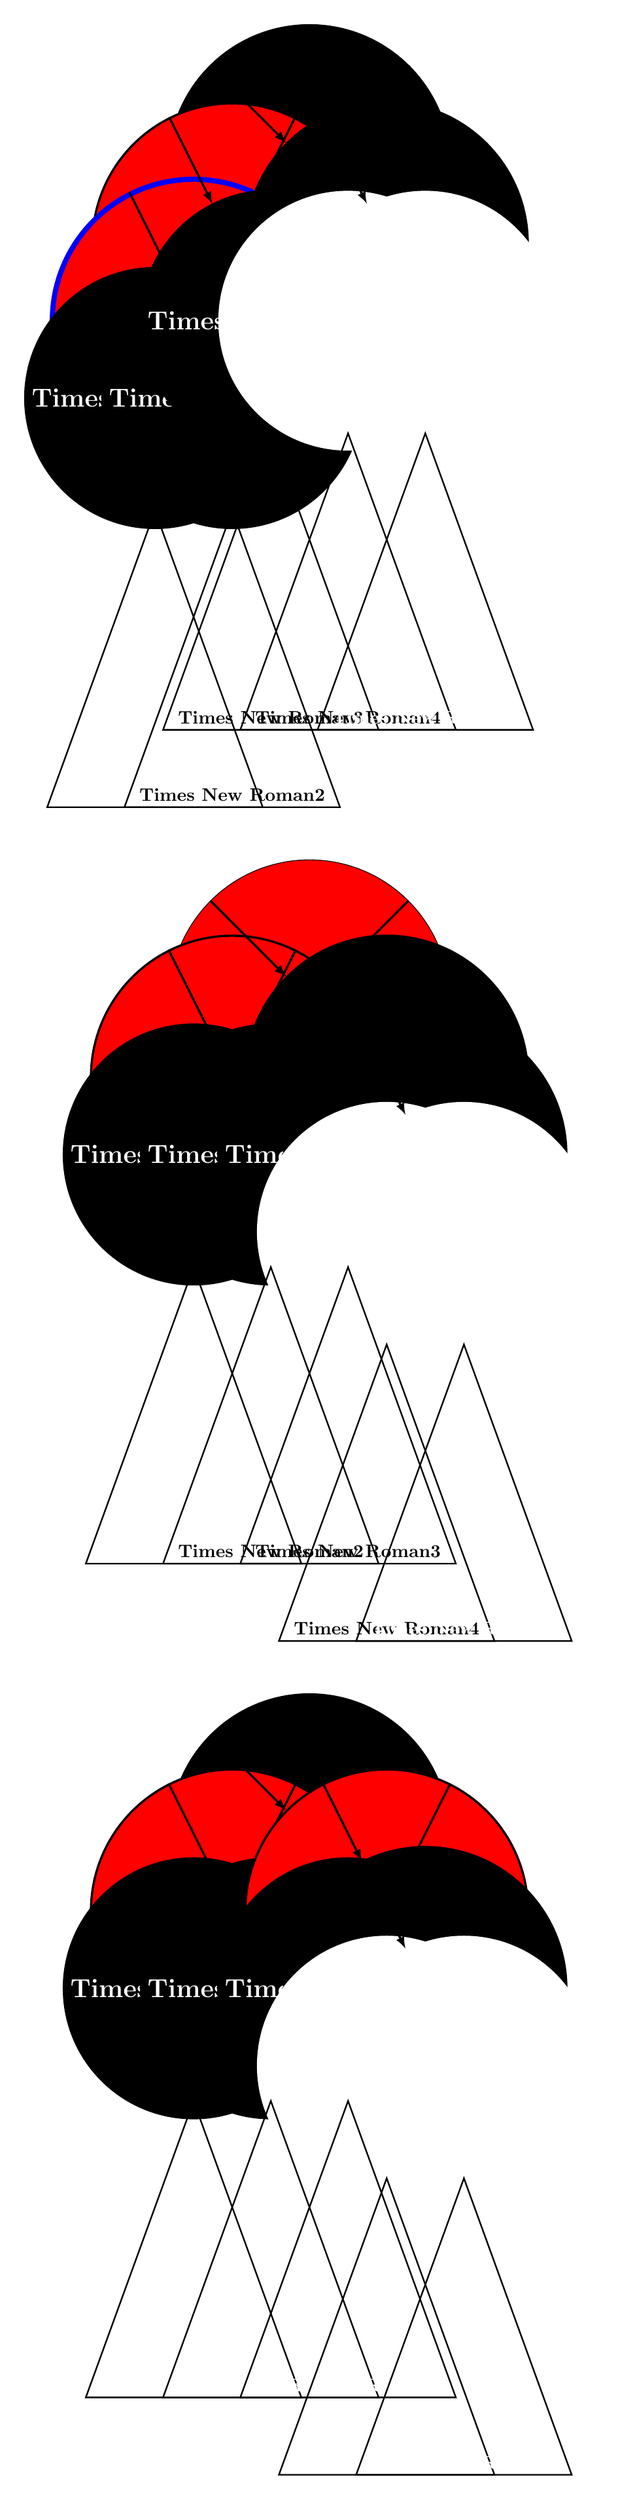
\begin{tikzpicture}
    \matrix[row sep=1cm, column sep=1cm] {
        \node[circlenode, fill=black] {G}
        child[real edge] {node[circlenode, fill=red] {P}
                child[real edge] {node[circlenode, fill=red, draw=blue, line width = 0.1cm] {N}
                        child[real edge] {node[circlenode, fill=black] (tree1){}}
                        child[real edge] {node[circlenode, fill=black] (tree2){}}
                    }
                child[real edge] {node[circlenode, fill=black] (tree3){}}
            }
        child[missing]
        child[real edge] {node[circlenode, fill=black] {U}
                child[real edge] {node[circlenode, draw=none, fill=white] (tree4){}}
                child[real edge] {node[circlenode, draw=none, fill=white] (tree5){}}
            };

        \node[trinode, below=-0.4cm of tree1, text = white] {1};
        \node[trinode, below=-0.4cm of tree2, text = black] {2};
        \node[trinode, below=-0.4cm of tree3, text = black] {3};
        \node[trinode, below=-0.4cm of tree4, text = black] {4};
        \node[trinode, below=-0.4cm of tree5, text = white] {5};

        \\

        \node[circlenode, fill=red] {P}
        child[real edge] {node[circlenode, fill=red] {N}
                child[real edge] {node[circlenode, fill=black] (tree1){}}
                child[real edge] {node[circlenode, fill=black] (tree2){}}
            }
        child[missing]
        child[real edge] {node[circlenode, fill=black] {G}
                child[real edge] {node[circlenode, fill=black] (tree3){}}
                child[real edge] {node[circlenode, fill=black] {U}
                        child[real edge] {node[circlenode, draw=none, fill=white] (tree4){}}
                        child[real edge] {node[circlenode, draw=none, fill=white] (tree5){}}
                    }
            };

        \node[trinode, below=-0.4cm of tree1, text = white] {1};
        \node[trinode, below=-0.4cm of tree2, text = black] {2};
        \node[trinode, below=-0.4cm of tree3, text = black] {3};
        \node[trinode, below=-0.4cm of tree4, text = black] {4};
        \node[trinode, below=-0.4cm of tree5, text = white] {5};

        \\

        \node[circlenode, fill=black] {P}
        child[real edge] {node[circlenode, fill=red] {N}
                child[real edge] {node[circlenode, fill=black] (tree1){}}
                child[real edge] {node[circlenode, fill=black] (tree2){}}
            }
        child[missing]
        child[real edge] {node[circlenode, fill=red] {G}
                child[real edge] {node[circlenode, fill=black] (tree3){}}
                child[real edge] {node[circlenode, fill=black] {U}
                        child[real edge] {node[circlenode, draw=none, fill=white] (tree4){}}
                        child[real edge] {node[circlenode, draw=none, fill=white] (tree5){}}
                    }
            };

        \node[trinode, below=-0.4cm of tree1, text = white] {1};
        \node[trinode, below=-0.4cm of tree2, text = white] {2};
        \node[trinode, below=-0.4cm of tree3, text = white] {3};
        \node[trinode, below=-0.4cm of tree4, text = white] {4};
        \node[trinode, below=-0.4cm of tree5, text = white] {5};

        \\
    };
\end{tikzpicture}
\end{document}
